\section{Details of Numerical Models for ASR Simulation}

\subsection{Geometry of Numerical Models}

Figure \ref{fig:model} shows the geometry of the model, which is in dimension of 100 x 100 x 100mm. Numbers of elements around 120000. Average diameter of meshed element is around 2mm.

\begin{figure}[ht!]
\centering
\begin{subfigure}{.5\textwidth}
  \centering
  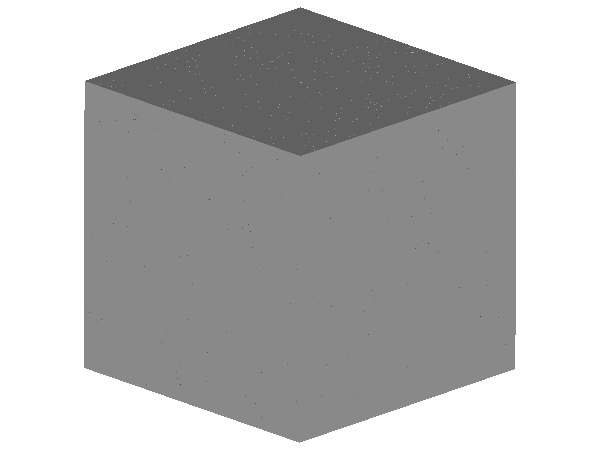
\includegraphics[width=.6\linewidth]{Files/exp_3D/Undamaged.png}
  \caption{3D model in dimension 100x100x100mm}
\end{subfigure}%
\begin{subfigure}{.5\textwidth}
  \centering
  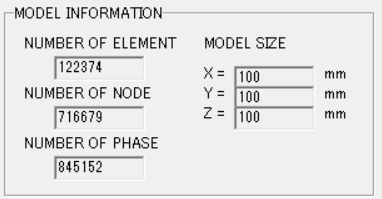
\includegraphics[width=.8\linewidth]{Files/Model/A30.png}
  \caption{Model Detail for 30\% Coarse Aggregate Case}
\end{subfigure}
\caption{Numerical Model for Expanding Simulation}
\label{fig:model}
\end{figure}

\subsection{Coarse Aggregate of Numerical Models}

To analysis the behavior of concrete with different coarse aggregate volume ratio, 15\% coarse aggregate model(Figure \ref{fig:A15_model}) and 30\% coarse aggregate model(Figure \ref{fig:A30_model}) are built for simulation.

\begin{figure}[ht!]
\centering
\begin{subfigure}{.5\textwidth}
  \centering
  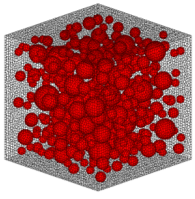
\includegraphics[width=.4\linewidth]{Files/Aggregate/A15.png}
  \caption{15\% Coarse Aggregate}
  \label{fig:A15_model}
\end{subfigure}%
\begin{subfigure}{.5\textwidth}
  \centering
  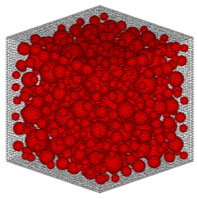
\includegraphics[width=.4\linewidth]{Files/Aggregate/A30.png}
  \caption{30\% Coarse Aggregate}
  \label{fig:A30_model}
\end{subfigure}
\caption{Coarse Aggregate Percentage}
\label{fig:Aggregate_Percentage}
\end{figure}

\subsection{ASR Reactive Coarse Aggregate Ratio}

To analysis the behavior of concrete with different ASR reactive coarse aggregate ratio, 25\% ASR reactive coarse aggregate ratio model and 25\% ASR reactive coarse aggregate ratio model are built for 30\% aggregate case.

\begin{figure}[!h]
\centering
\begin{subfigure}{.5\textwidth}
  \centering
  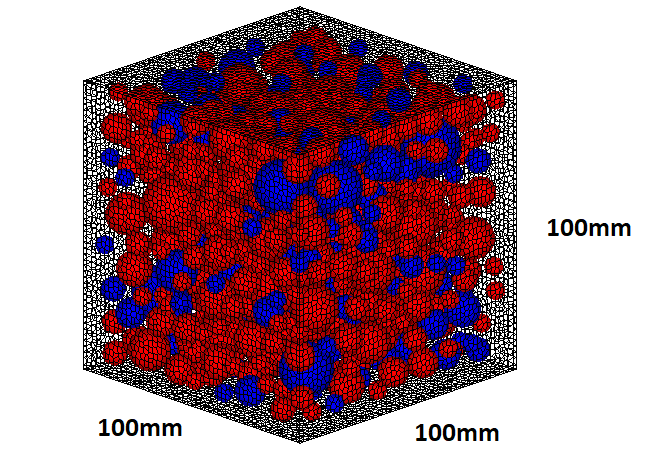
\includegraphics[width=.5\linewidth]{Files/Aggregate/A30P75.png}
  \caption{30\% Coarse Aggregate with 75\% ASR Reactive Aggregate}
\end{subfigure}%
\begin{subfigure}{.5\textwidth}
  \centering
  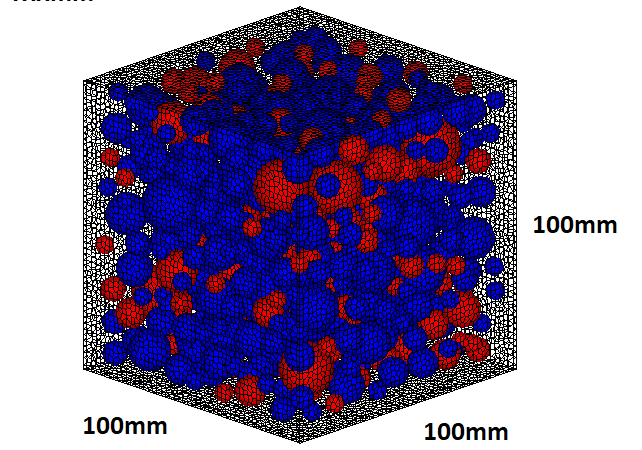
\includegraphics[width=.5\linewidth]{Files/Aggregate/A30P25.png}
  \caption{30\% Coarse Aggregate with 25\% ASR Reactive Aggregate}
\end{subfigure}
\caption{25\% and 75\% ASR Reactive Aggregate Ratio Model}
\label{fig:Aggregate_Percentage}
\end{figure}

\subsection{Boundary Conditions}

\subsubsection{Boundary Condition During ASR Expansion}

During ASR Expansion, no confinements are added to the boundary elements. Models expanse freely in all directions.

\subsubsection{Boundary Conditions During Uni-axial Loading Test}

Figure \ref{boundary} shows the boundary condition of simulation models for uni-axial loading test.

\begin{figure}[h!]
  \centering
  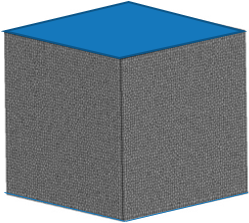
\includegraphics{Files/Background/LOAD.png}
  \caption{Top and Bottom Boundary in Loading}
  \label{boundary}
\end{figure}

In the case of fixed boundary condition, displacement in all directions are assumed as 0 at the bottom. Displacement in horizontal directions are all assumed as 0 at the top, and displacement in vertical direction is increased by 0.02mm downward at each loading step.

In the case of free boundary condition, all boundary elements able to move freely in horizontal direction except 2 center elements in top and bottom are fixed in horizontal direction, to prevent the sliding of whole model during loading. Same as fixed boundary condition cases, displacement in vertical direction is increased by 0.02mm downward at each loading step for top boundary elements.

Loading is applied until the maximum compressive strength is reached.

\subsection{Initial Strain Given For ASR Expansion}

To analysis the relationship of concrete behavior and mechanical properties with expansion amount, initial strain is given between reactive aggregate and mortar.

\begin{table}[ht!]
\centering
\begin{tabular}{ ||p{2cm}|p{2cm}|p{2cm}|p{2cm}|p{2cm}|| }
 \hline
 Aggregate Ratio[\%] &  Reactive Aggregate Ratio[\%] & Boundary Condition & Initial Strain (Each Step) & Expanding Steps \\ [0.5ex]
 \hline\hline
 15 & 75 & Fix & 0 & 0 \\
 15 & 75 & Fix & 0.0002 & 20 \\
 15 & 75 & Fix & 0.0005 & 20 \\
 15 & 75 & Fix & 0.001 & 20 \\
 15 & 75 & Fix & 0.002 & 20 \\
 15 & 75 & Fix & 0.003 & 20 \\

 15 & 75 & Free & 0 & 0 \\
 15 & 75 & Free & 0.0002 & 20 \\
 15 & 75 & Free & 0.0005 & 20 \\
 15 & 75 & Free & 0.001 & 20 \\
 15 & 75 & Free & 0.002 & 20 \\

 30 & 75 & Fix & 0 & 0 \\
 30 & 75 & Fix & 0.0002 & 20 \\
 30 & 75 & Fix & 0.0005 & 20 \\
 30 & 75 & Fix & 0.001 & 20 \\
 30 & 75 & Fix & 0.002 & 20 \\
 30 & 75 & Fix & 0.003 & 20 \\

 30 & 75 & Free & 0 & 0 \\
 30 & 75 & Free & 0.0002 & 20 \\
 30 & 75 & Free & 0.0005 & 20 \\
 30 & 75 & Free & 0.001 & 20 \\
 30 & 75 & Free & 0.002 & 20 \\

 30 & 25 & Fix & 0 & 0 \\
 30 & 25 & Fix & 0.001 & 20 \\
 30 & 25 & Fix & 0.002 & 20 \\
 30 & 25 & Fix & 0.004 & 20 \\
 30 & 25 & Fix & 0.006 & 20 \\  [0.5ex]
 \hline
\end{tabular}
\caption{ASR Models}
\label{table:ASR_MODELS}
\end{table}

%*******10********20********30********40********50********60********70********80
